\documentclass[a4paper,12pt]{article}
\usepackage[french]{babel}
\usepackage[T1]{fontenc}
\usepackage[utf8]{inputenc}
\usepackage{textcomp}
\usepackage{graphicx}
\usepackage{xcolor}
\usepackage[a4paper,left=2.5cm,right=2.5cm,top=2cm,bottom=2cm]{geometry}
\usepackage{amsmath}
\usepackage{amssymb}
\usepackage{pifont}
\usepackage{subfig}
%\usepackage{siunitx}
\usepackage{xcolor}
%\usepackage{bbm}

%opening
\title{Documentation du logiciel de post-processing de Liggghts \\ Avancement du d\'evelopement}
\author{F. G.}
\date{\today}

\begin{document}
\maketitle
\tableofcontents
\newpage

\section{Historique}
28/03/2011 : cr\'eation de la compression de base pour les dump atomiques (positions des atomes, rayons etc. La compression se fait sur les valeurs \`a chaque timestep. Si au cours du temps (sur le fichier complet), le nombre de valeur pris par un type de donn\'ee est fini (1, 2, 4 ou 16), les donn\'ees sont compress\'ees en allouant un nombre de bit inf\'erieur \`a l'octet pour la donn\'ee en question.\\
12/09/2011 : addition de la compression des dump de force sur les triangle de mesh. La compression se base le regroupement effectu\'e auparavant dans le programme de post-processing des donn\'ees de force et des donn\'ees de dump atomique. Pour une backward compatibility correcte, les modifications \`a cette date sont en \textcolor{red}{rouge} dans ce fichier. Une extension apport\'ee \`a la compression est la v\'erification s'il existe des modifications des donn\'ees d'un timestep \`a l'autre, et l'ajout de type de donn\'ees en lien avec cela.

\begin{table}
\begin{tabular}{|l|l|c|p{6cm}|}\hline
Version majeure & Version mineure & Date & Modifications \\ \hline
1 & 0 & 28/03/2011 & Cr\'eation de la compression des L dump (dump atomique de base) \\ \hline
2 & 0 & 12/09/2011 & Ajout de la compression des F dump (dump de force sur objet) \\ \hline
2 & 1 & 16/06/2012 & Correction d'un bug lors de l'\'ecriture des formats d\'enombrables (2 et +) \\ \hline
2 & 5 & 05/2014 & Modifications internes assez importantes : Le coarse-graining passe en classe dump, les identifiants ont leur classe \`a part plus modulable (IDS), la classe Writing permet un \'ecriture plus modulable. \\ \hline
%2 & 5 & 02/11/2013 & \'Elimination des bouts de codes pas finis. Modifications des chainforces \\ \hline
\end{tabular}
\caption{Version importantes de PostProcessing}
\end{table}

\begin{figure}
 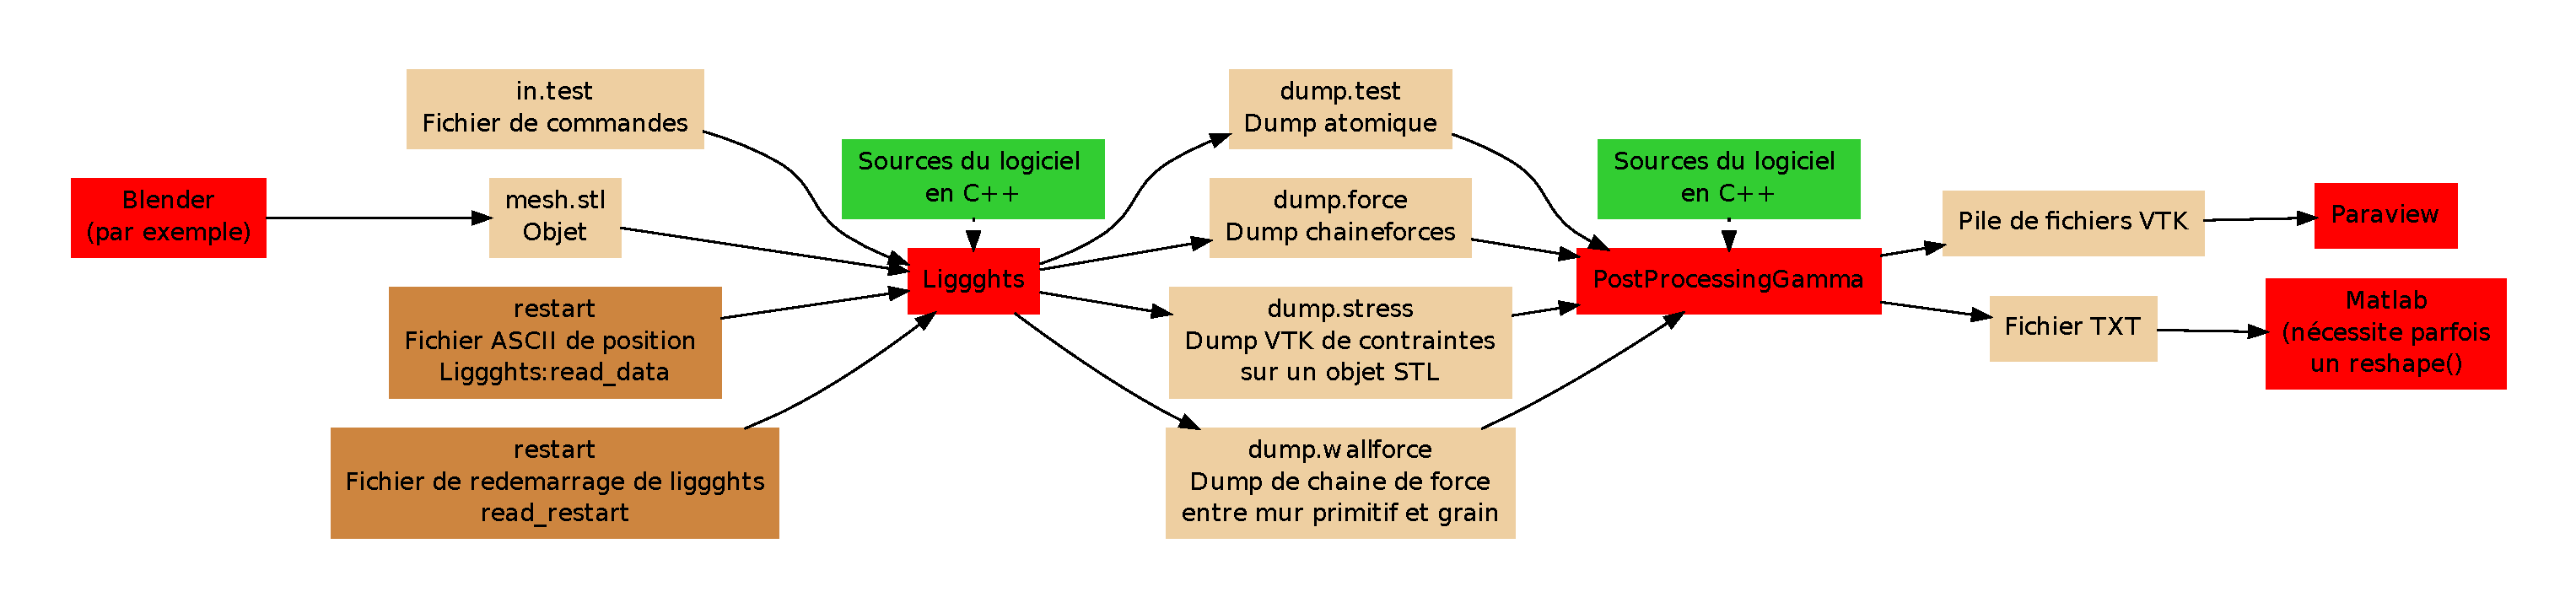
\includegraphics[width=\linewidth]{Liggghts.pdf}
 \caption{Sch\'ema de la cha\^ine de fonctionnement de Liggghts.}
 \label{ClassesCPP}
\end{figure}

\begin{figure}
 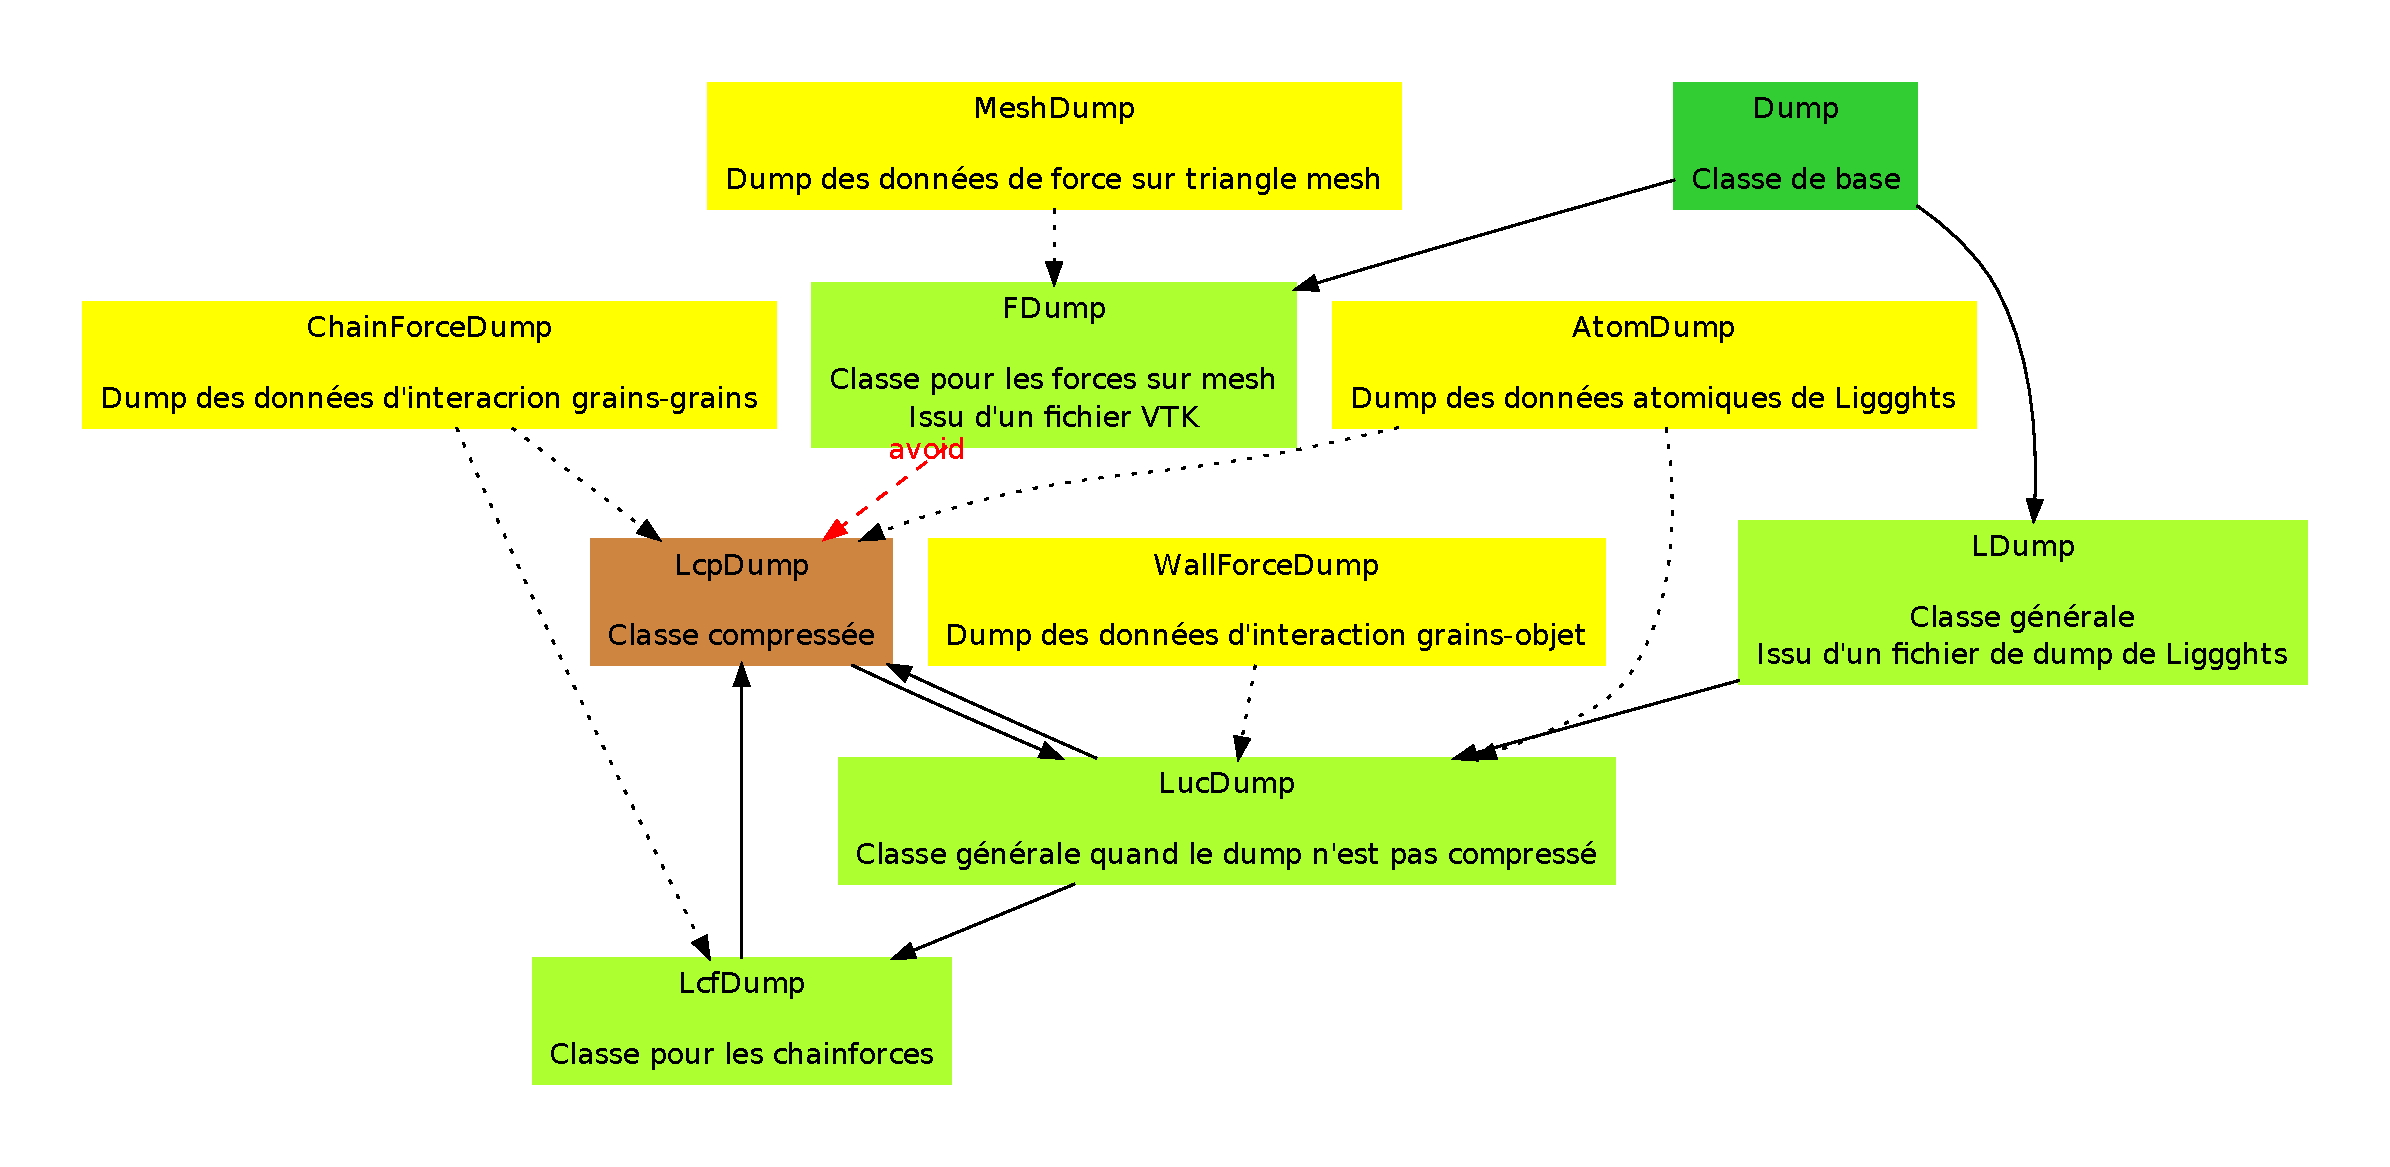
\includegraphics[width=\linewidth]{Dump.pdf}
 \caption{Sch\'ema des relations de classes de dumps dans PostProcessing \textcolor{red}{OUTDATED}}
 \label{ClassesCPP}
\end{figure}




\newpage
\section{Fonctionnement g\'en\'eral}
Le dernier argument de la ligne de commande est le nom du fichier de donn\'ees \`a lire. Il s'ag\^it d'un dump de donn\'ees atomique (donn\'ees pour chaque atome), not\'e ATOMDUMP dans la suite, et qui correspond \`a une variable de classe LDump dans le code C++ (plus pr\'ecis\'ement LucDump si c'est un dump non compress\'e par le logiciel de PostProcessing, LcpDump si c'est un dump compress\'e). Voir la figure \ref{ClassesCPP} pour les relations entre les classes du code source.

Lorsque l'argument \verb{--vtk{ est donn\'e, le dernier argument doit \^etre un fichier VTK unique contenant les donn\'ees d'interactions entre un objet stl (mesh) et les grains (ie. les forces sur chaque triangle). Il s'ag\^it alors d'un dump de classe C++ FDump.

Lorsque l'argument \verb{--chainforce{ est donn\'e dans la ligne de commande, les 2 derniers arguments deviennent les fichiers de donn\'ees. L'avant-dernier argument est un fichier ATOMDUMP, le dernier argument contient les chaines de forces, not\'e CFDUMP dans la suite, et correspond \`a une variable de classe LcfDump dans le code C++.

Dans certains cas (\verb{--wallchainforce{, cf partie suivante), les 3 derniers arguments peuvent \^etre des dumps, pour prendre en compte les chaines de forces primitivewall--grain, qui ne sont pas incluses dans les CFDUMP. 

\bigskip

Pour la lecture du fichier, g\'en\'eralement, une premi\`ere passe est effectu\'ee pour rep\'erer la position de d\'epart des donn\'ees de chaque pas de temps. Ces donn\'ees sont stock\'ees dans un fichier *.tmp qui permet une lecture plus rapide la fois suivante lorsque le m\^eme fichier de dump est r\'eutilis\'e. Par contre, il faut r\'eg\'en\'erer le tmp si le dump est modifi\'e ou lors de l'utilisation de CFDUMP (c'est fait automatiquement normalement). 

A priori il est pr\'ef\'erable de toujours utiliser les arguments \verb+--v2+ et \verb+--rebuild+ \`a partir de maintenant lorsque l'on utilise des chaines de force.

\newpage
\section{Exemple de quelques commandes ...}
\subsection{Commandes g\'en\'erales}
\verb+$ PostProcessingGamma --help null+ : Liste tous les arguments possibles pour PostProcessing. 

\verb+$ PostProcessingGamma --dump2vtk --w/id --w/rayon ATOMDUMP+ : transforme un dump en une s\'erie de fichiers VTK lisibles par paraview avec un champ contenant les ID et un champ contenant les rayons des atomes.

\verb+$ PostProcessingGamma --chainforce --v2 --rebuild ATOMDUMP CFDUMP+ : pour sortir des VTK affichant les chaines de forces dans paraview.

\subsection{Pour un coarse graining correct}
Pour le coarse-graining, il peut y avoir jusqu'\`a 3 dump \`a fournir :
\begin{itemize}
\item Coarse-graining de vitesses et compacit\'es : un seul dump de type Ldump avec les positions des atomes (appel\'e ATOMDUMP dans la suite).
\item Coarse-graining de contrainte : 2 dump avec l'argument \verb{--chainforce{. Le dernier argument est un dump de type TCF (CFdump, CFDUMP dans la suite) et contient les forces particules-particules, l'avant dernier est un argument de type TL (Ldump) et contient les positions des atomes. Le coarse graining de vitesse est automatiquement effectu\'e en m\^eme temps, mais il ne faut pas trop s'y fier je pense ...
\item Coarse-graining de grains cylindriques polydisperses (2D) : utiliser l'argument \verb{--polydisperse2D{.
\item Coarse-graining incluant les interactions avec le mur : 3 dump avec les arguments \verb{--chainforce --wallchainforce x x x{. Le dernier et l'avant dernier argument sont les dumps indiqu\'e au point pr\'ec\'edent, l'avant-avant dernier argument est un dump de type TL (LDump, WALLFORCEDUMP dans la suite) contenant les interactions grains-cylindre (ne fonctionne qu'avec un cylindre pour l'instant). 
\end{itemize}
\bigskip 
Probl\`emes \`a \'eviter : 
\begin{itemize}
\item Faire un clean de tous les tmp pour les dump utilis\'es (par mesure de pr\'ecaution, les tmp n'enregistrant pas les types de dump \c ca peut causer probl\`eme).
\item Les timestep de tous les dump devraient \^etre identiques pour \'eviter les probl\`emes (m\^eme si une petite v\'erification est faite pour les 
\item Il est conseill\'e d'utiliser toujours \verb{--winsphere{ en granulaire avec le ATOMDUMP, et de ne pas l'utiliser sinon (permet une mesure pr\'ecise de la compacit\'e). ATTENTION : il ne faut donc pas se fier aux compacit\'es dans les coarse-graining de contrainte.
\item Les contraintes sont TOUTES avec un signe MOINS (les donn\'ees extraites sont donc $\sigma_{ij}=P\delta_{ij} - \tau_{ij}$.
\end{itemize}

Exemple de commandes : 
\begin{verbatim}
$ PostProcessingGamma --coarse-graining 120 3 120 --use-box -0.1 0.1 -0.007 0.007 0 0.2 \ 
--winsphere --v2 ATOMDUMP

$ PostProcessingGamma --chainforce --coarse-graining 120 3 120 \ 
--use-box -0.1 0.1 -0.007 0.007 0 0.2 --periodicity ATOMDUMP CFDUMP

$ PostProcessingGamma --chainforce --coarse-graining 120 3 120 \
--use-box -0.1 0.1 -0.007 0.007 0 0.2 --v2  \
--wallchainforce 0 0.08 0.0025 WALLFORCEDUMP ATOMDUMP CFDUMP
\end{verbatim}

Rappel des arguments des options : 
\begin{verbatim}
--coarse-graining 120 3 120 : nb de boites en x, y, z
--chainforce : pas d'arguments
--use-box -0.1 0.1 -0.7 0.7 0 0.2 : limites de l'espace en -x, +x, -y, +y, -z, +z
--periodicity : le CFDUMP indique si les interactions traversent 
                 une condition limite periodique. (cf le tableau 1)
--v2 : indique un liggghts version 2 (qques diff\'erences de syntaxe ...). 
                 Implique periodicity
--wallchainforce 0 0.08 0.0025 : position x, position z et rayon du cylindre 
                 (rayon unused pour l'instant ...).
\end{verbatim}


%===============================================================
\newpage
\section{Extraction des donn\'ees : la classe writing.}
La classe Writing g\`ere les fonctions particuli\`eres d'\'ecriture des donn\'ees dans les diff\'erents formats. \`A chaque d\'emarrage de PostProcessing, elle est initialis\'ee avec les informations suivantes : 
\begin{itemize}
\item Le ou les formats de sortie : \begin{itemize}
  \item vtk : format pour lecture paraview. 
  \item mat : format lisible avec matlab.
  \item ascii : format tableau ascii. \end{itemize}
\item Pour chaque format la liste des variables \`a \'ecrires (existantes a priori ou non).
\end{itemize}

\subsection{Fonctionnement}
Le principe est que lorsqu'une classe dump a besoin d'une \'ecriture, elle converse avec la classe Writing \`a travers un \'echange de signaux (Writing est en fait un thread s\'epar\'e). Donc Writing demande les infos donc il a besoin, et dump les charge en m\'emoire (si possible), et passe le pointeur \`a Writing. Sur les format VTK, qui ont 1 fichier par timestep, 1 seul est charg\'e \`a chaque fois. Par contre pour l'ascii et le mat, tout est charg\'e d'un coup ce qui peut \^etre probl\'ematique pour des gros fichiers.

\subsection{Compilation, ex\'ecution}
Pour compiler avec le support pour l'\'ecriture de fichiers matlab, il faut d\'efinir la macro MATLAB (id\'ealement dans le makefile), inclure les r\'epertoires d'include de matlab dans la compilation, dans le linkage inclure les r\'epertoires des librairies (a priori dynamiques) de matlab.
Ensuite, lors de l'ex\'ecution, il faut que la librairie dynamique matlab soit dans les r\'epertoires de recherche des librairies dynamiques (sous mac, il faut \'editer la variable environnement \$DYLD\_LIBRARY\_PATH).

\subsection{Parler avec la classe Writing}
En ligne de commande, l'argument apr\`es \verb+--write+ (ou \verb+--W+ qui est un raccourci) doit \^etre une cha\^ine de caract\`eres. Elle peut contenir des espaces, des retours \`a la ligne, des fabulations etc. qui seront ignor\'ees. La cha\^ine est ensuite process\'ee de la mani\`ere suivante : 
\begin{itemize}
\item Les textes entre accolades \{ \} sont des fonctions. Le principe est que le texte entre accolades est un nom de fonction, qui est appel\'e pour chaque variable suivante, en passant en outre le format d'\'ecriture rencontr\'e pr\'ec\'edemment s'il existe. Voir le tableau \ref{Writing_fonctions} pour les fonctions existantes.
\item Les textes entre crochets $\left [ \right ] $ se r\'ef\`erent aux formats d'\'ecriture. (e.g. \texttt{[+vtk], [-mat], [ascii]}). Un format pr\'ec\'ed\'e de $+$ est s\'el\'ectionn\'e, de $-$ est d\'es\'el\'ectionn\'e, de rien est conserv\'e dans le m\^eme \'etat (attention du coup). 
\item Le reste sont des variables, qui se r\'ef\`erent \`a la fonction ou \`a la classe pr\'ec\'edente. Les variables sont s\'epar\'ees par des virgules ou des points virgules. Il y a deux variables particuli\`eres : \begin{itemize}
\item \texttt{def} : charger les variables par d\'efaut pour le format en cours. Utile pour \'ecrire un format non charg\'e automatiquement.
\item \texttt{nodef} : ne pas charger les variables par d\'efaut. Utile pour modifier un format charg\'e automatiquement.
\end{itemize}\end{itemize}
Ce qui donne \texttt{"cfdump:mat [cfdump:mat] vx, pos, masse, atm:masse"}.

\begin{table}
\begin{tabular}{l|p{5cm}|p{5cm}}
Fonction & Effet & Exemple \\ \hline
\verb+{expand}+ & Les variables en interne s'expandent en variables de dimension 1 & \verb+[vtk]{expand}pos+ est comme \verb+[vtk]posx,posy,posz+
\end{tabular}
\caption{Fonctions d\'efinies pour l'instant}
\label{Writing_fonctions}
\end{table}

\subsection{Dimensions}
Chaque variable a une dimension. Les variables de base telles que d\'efinies dans la classe IDS sont toutes de dimension 1. Writing d\'efini des variables de dimension 2 (vecteur) et 3 (tenseur). Le principe est que les variables de dimensions $n>1$ se d\'ecomposent en variables de dimension $n-1$ en ajoutant d'abord $x$, puis $y$, puis $z$. 

\begin{itemize}
\item \textbf{vtk} 
\begin{itemize}
\item 1D  SCALARS
\item 2D  VECTORS
\item 3D  TENSORS
\end{itemize}
\item \textbf{mat}  Pour les matrices. 1e dimension : atome / contact / bo\^ite, 3e dimension : timestep, 2e dimension \begin{itemize}
\item 1D  1 sur la 2e dimension des matrices. 
\item 2D  3 sur la 2e dimension des matrices.
\item 3D  9 sur la 2e dimension des matrices.
\end{itemize}
\item \textbf{ascii}  L'\'ecriture ascii est un peu particuli\`ere. Si $v$ le nombre de variables \`a \'ecrire, $N_i$ est le nombre d'atomes / contacts / bo\^ites pour la variable $i$, $d_i$ la dimension de la variable $i$, $ts$ le nombre de ts.
\begin{itemize}
\item On ne peut avoir $ts>1$ AND $\exists i \left | d_i>1\ \text{AND}\ N_i>1 \right .$.
\item Si $ts=1$ AND $\forall i, d_i=1\ \text{AND}\ N_i=cst$, alors 1 seul fichier est \'ecrit (extension \verb+-ascii.txt+) contenant toutes les variables.
\item Sinon, on \'ecrit 1 fichier par variable (quelle que soit leur dimension).
\end{itemize}
\end{itemize}

NB : l'utilisation de la fonction \verb+{expand}+ rend toutes les variables de dimension 1 en interne, permettant l'\'ecriture d'un seul fichier ascii tout en utilisant les noms raccourcis par exemple. 


\begin{table}
\begin{tabular}{|l|c|}\hline
Variables de Writing n'existant pas en IDS & Dimension \\\hline
\verb+general1D+ (Controle seulement) & 1\\
\verb+pos+ & 2\\
\verb+v+ & 2\\
\verb+f+ & 2\\
\verb+omega+ & 2 \\
\verb+sigma+ & 3 \\
\verb+cff+ & 2 \\
\verb+cfforce+ & 2 \\
\verb+sigmak+ & 3 \\
\verb+sigmatot+ & 3 \\
\verb+forcewall+ & 2 \\\hline
\end{tabular}
\caption{Variables compatibles avec chaque classe. En Vert, extrait obligatoirement. En rouge, raccourci (vecteurs), en bleu, raccourci (tenseur)}
\end{table}

\newpage
\section{La classe IDS}
La classe IDS d\'efinie les types de donn\'ees pour tous les fichiers de dump. Elle est de plus extensible et peut ajouter des donn\'eese qu'elle ne conna\^it pas avec les propri\'et\'es de base. Chaque variable a un nom de base (en majuscule) et 1 ou plusieurs alias.

\begin{table}
\begin{tabular}{|l|l|c|c|}\hline
Type & Classe associ\'ee & ID min & ID max \\ \hline
TL & LDump & 1 & 63 \\\hline
TCF & LcfDump & 64 & 127 \\\hline
TF & FDump & 128 & 191 \\\hline
TCOARSE & CoarseDump & 192 & 254 \\\hline
TNONE  & & 1 & 254 \\\hline
\end{tabular}
\caption{Les diff\'erents types de donn\'ees d\'efinis par IDS et leur range d'identifiants. NB: Les ID sont d\'efinis en CHAR et sont donc limit\'es \'a 256 valeurs}
\end{table}

\begin{table}
\begin{minipage}{\linewidth}
\renewcommand{\footnoterule}{}
\renewcommand{\thefootnote}{\alph{footnote}}
\begin{tabular}{|c|c|c|c|l|} \hline
  \textbf{Constante c} & \textbf{Int. c} & \textbf{Txt dump} & \textbf{Nom commun} & \textbf{Format} \\ \hline
   ID      &1   & id & Identifiant atome & UInt\\ \hline
   TYPE    &2   & type & Type d'atome      & UChar\\ \hline
   POSX    &3   & x & Position x        & Float / Double\\ \hline
   POSY    &4   & y & Position y       & Float / Double\\ \hline
   POSZ    &5   & z & Position z        & Float / Double\\ \hline
   VX      &6   & vx & Vitesse x         & Float / Double\\ \hline
   VY      &7   & vy & Vitesse y         & Float / Double\\ \hline
   VZ      &8   & vz & Vitesse z         & Float / Double\\ \hline
   RAYON   &9 & radius  & Rayon             & Float / Double\\ \hline
   FX      &10  & fx & Force x           & Float / Double\\ \hline
   FY      &11  & fy &Force y           & Float / Double\\ \hline
   FZ      &12  & fz & Force z           & Float / Double\\ \hline   
   MASSE      &13  & mass & Masse           & Float / Double  \footnotemark[2]\\ \hline
   OMEGAX      &14  & omegax & Vitesse angulaire x \footnotemark[3]  & Float / Double \footnotemark[2] \\ \hline
   OMEGAY      &15  & omegay & Vitesse angulaire y  \footnotemark[3]  & Float / Double \footnotemark[2]\\ \hline
   OMEGAZ      &16  & omegaz & Vitesse angulaire z  \footnotemark[3]  & Float / Double \footnotemark[2]\\ \hline
   SIGMA$[$XYZ$][$XYZ$]$      &17 \`a 25 & sigma$[$xyz$][$xyz$]$ & Contraintes \footnotemark[3] & Float / Double  \footnotemark[2]\\ \hline
   FORCEWALLX   &26  & f\_force\_cyl$[$1$]$ & Force particule/mur           & Float / Double \footnotemark[2]\\ \hline
   FORCEWALLY   &27  & f\_force\_cyl$[$2$]$ & Force particule/mur           & Float / Double \footnotemark[2]\\ \hline
   FORCEWALLZ   &28  & f\_force\_cyl$[$3$]$ & Force particule/mur           & Float / Double \footnotemark[2]\\ \hline
   ATMPRESSURE   &29  & atmpressure & Pression par atome   & Float / Double \footnotemark[2]\\ \hline
    \textbf{UNKNOWN} &255 & RESERVED         & RESERVED &\\ \hline
 \end{tabular}
 \footnotetext[1] {Ne doit pas \^etre compress\'e.}
 \footnotetext[2] {Compression non r\'eellement test\'ee.}
 \footnotetext[3] {Unused. Leur utilisation devrait \^etre v\'erifi\'ee si besoin.} 
 \end{minipage}
\caption{Table des types de donn\'ees de type TL d\'efinis au \today.}\label{Types}
\end{table}

\begin{table}
\begin{minipage}{\linewidth}
\renewcommand{\footnoterule}{}
\renewcommand{\thefootnote}{\alph{footnote}}
\begin{tabular}{|c|c|c|c|l|} \hline
  \textbf{Constante c} & \textbf{Int. c} & \textbf{Txt dump} & \textbf{Nom commun} & \textbf{Format} \\ \hline
    \color{green} CFID1 & 64 & c\_cout$[$1$]$ & ID atm1 & UInt\\ \hline
    \color{green}CFID2 & 65 & c\_cout$[$2$]$ &ID atm2 & UInt\\ \hline
    \color{green}CFFORCEX & 66 & c\_cout$[$3$]$ / c\_cout$[$4$]$ \footnotemark[4] & Force x du lien &Float / Double\\ \hline
    \color{green}CFFORCEY & 67 & c\_cout$[$4$]$ / c\_cout$[$5$]$ \footnotemark[4] & Force y du lien & Float / Double\\ \hline
    \color{green}CFFORCEZ & 68 & c\_cout$[$5$]$ / c\_cout$[$6$]$ \footnotemark[4] &Force z du lien & Float / Double\\ \hline
    \color{green}CFMAG & 69 & Construit &Magnitude du lien & \\ \hline
    \color{green}CFR & 70 & Construit & Lien en polaire \footnotemark[1] & \\ \hline
    \color{green}CFTHETA & 71 & Construit & Lien en polaire\footnotemark[1] & \\ \hline
    \color{green}CFPHI & 72 & Construit & Lien en polaire\footnotemark[1] & \\ \hline
    \color{green}CFX & 73 & Construit &Position x du lien\footnotemark[1]& \\ \hline
    \color{green}CFY & 74 & Construit &Position y du lien\footnotemark[1]& \\ \hline
    \color{green}CFZ & 75 & Construit &Position z du lien\footnotemark[1]& \\ \hline
    \color{green}CFPERIOD & 76 & c\_cout$[$3$]$ \footnotemark[4] &P\'eriodicit\'e du lien & UChar\\ \hline   
    \color{green}CFID1X & 77 & c\_contacts$[$1$]$\footnotemark[5] & Pos x atm 1 du contact & Float / Double\\ \hline
    \color{green}CFID1Y & 78 & c\_contacts$[$2$]$\footnotemark[5] & Pos y atm 1 du contact & Float / Double\\ \hline
    \color{green}CFID1Z & 79 & c\_contacts$[$3$]$\footnotemark[5] & Pos z atm 1 du contact & Float / Double\\ \hline
    \color{green}CFID2X & 80 & c\_contacts$[$4$]$\footnotemark[5] & Pos x atm 2 du contact & Float / Double\\ \hline
    \color{green}CFID2Y & 81 & c\_contacts$[$5$]$\footnotemark[5] & Pos y atm 2 du contact & Float / Double\\ \hline
    \color{green}CFID2Z & 82 & c\_contacts$[$6$]$\footnotemark[5] & Pos z atm 2 du contact & Float / Double\\ \hline
     \textbf{UNKNOWN} &255 & RESERVED         & RESERVED &\\ \hline
 \end{tabular}
 \footnotetext[1] {Ne doit pas \^etre compress\'e.}
 \footnotetext[2] {Compression non r\'eellement test\'ee.}
 \footnotetext[3] {Unused. Leur utilisation devrait \^etre v\'erifi\'ee si besoin.} 
 \footnotetext[4] {Dans les version r\'ecentes de liggghts, la p\'eriodicit\'e est indiqu\'e dans la coordonn\'ee 3 (CFPERIOD). Les autres c\_cout sont donc d\'ecall\'es de 1.}
 \footnotetext[5] {Peut entrer en conflit avec CFFORCE et CFID. Il faut faire attention.} 
\end{minipage}
\caption{Table des types de donn\'ees de type TCF d\'efinis au \today.}\label{Types}
\end{table}

\begin{table}
\begin{minipage}{\linewidth}
\renewcommand{\footnoterule}{}
\renewcommand{\thefootnote}{\alph{footnote}}
\begin{tabular}{|c|c|c|c|l|} \hline
  \textbf{Constante c} & \textbf{Int. c} & \textbf{Txt dump} & \textbf{Nom commun} & \textbf{Format} \\ \hline
   \color{red} PRESSURE & 128 & pressure & Pression & float \\ \hline
   \color{red}SHEARSTRESS & 129 & shearstress & Cisaillement & float \\ \hline
   \color{red}FORCEX & 130 & forcesTri\footnotemark[1]  &Force X & float \\ \hline
   \color{red}FORCEY & 131 & forcesTri\footnotemark[1]  & Force Y & float \\ \hline
   \color{red}FORCEZ & 132 & forcesTri\footnotemark[1]  & Force Y & float \\ \hline
   \color{red}NORMALEX & 133 & normales  & Normale X & float \\ \hline
   \color{red}NORMALEY & 134 & normales & Normale Y & float \\ \hline
   \color{red}NORMALEZ & 135 & normales &Normale Z & float \\ \hline
   \color{red}POINTX & 136 & POINTS & Point X & float \\ \hline
   \color{red}POINTY & 137 & POINTS & Point Y & float \\ \hline
   \color{red}POINTZ & 138 & POINTS & Point Z & float \\ \hline
   \color{red}POLY1 & 139 & POLYGONS & Nb de sommet du polygone & Int \\ \hline
   \color{red}POLY2 & 140 & POLYGONS & Sommet 1 & Int \\ \hline
   \color{red}POLY3 & 141 & POLYGONS & Sommet 2 & Int \\ \hline
   \color{red}POLY4 & 142 & POLYGONS & Sommet 3 & Int \\ \hline 
   \color{red}STRESSX & 143 & stress\footnotemark[2]  &Force X & float \\ \hline
   \color{red}STRESSY & 144 & stress\footnotemark[2]  &Force Y & float \\ \hline
   \color{red}STRESSZ & 145 & stress\footnotemark[2]  &Force Y & float \\ \hline
   \color{red}CENTREX & 146 & CELL\footnotemark[2]  &  Normale X & float \\ \hline
   \color{red}CENTREY & 147 & CELL\footnotemark[2]  & Normale Y & float \\ \hline
   \color{red}CENTREZ & 148 & CELL\footnotemark[2]  & Normale Z & float \\ \hline
   \textbf{UNKNOWN} & 255 & RESERVED         & RESERVED &\\ \hline
\end{tabular}
 \footnotetext[1] {Extraites d'une modification des sources de Liggghts 1. Plus utilis\'es.}
 \footnotetext[2] {Pour la version 2 de liggghts. La commande \texttt{--rebuild} permet de reconstruire FORCE$[$XYZ$]$ et d'autres choses \`a partir des donn\'ees de v2.}
\end{minipage}
\caption{Table des types de donn\'ees de type TF d\'efinis au \today~pour les FDump (dump de force sur les triangles d'un mesh, lus dans un fichier VTK).}
\end{table}


idname[192]="COARPHI" ;      idname[193]="COARATM" ;      idname[194]="COARCONTACTS" ; idname[195]="COARRAD" ;
idname[196]="COARSIGKXX" ;   idname[197]="COARSIGKXY" ;   idname[198]="COARSIGKXZ" ;
idname[199]="COARSIGKYX" ;   idname[200]="COARSIGKYY" ;   idname[201]="COARSIGKYZ" ;
idname[202]="COARSIGKZX" ;   idname[203]="COARSIGKZY" ;   idname[204]="COARSIGKZZ" ;
idname[205]="COARSIGTOTXX" ; idname[206]="COARSIGTOTXY" ; idname[207]="COARSIGTOTXZ" ;
idname[208]="COARSIGTOTYX" ; idname[209]="COARSIGTOTYY" ; idname[210]="COARSIGTOTYZ" ;
idname[211]="COARSIGTOTZX" ; idname[212]="COARSIGTOTZY" ; idname[213]="COARSIGTOTZZ" ;


\begin{table}
\begin{minipage}{\linewidth}
\renewcommand{\footnoterule}{}
\renewcommand{\thefootnote}{\alph{footnote}}
\begin{tabular}{|c|c|c|c|l|} \hline
  \textbf{Constante c} & \textbf{Int. c} & \textbf{Txt dump} & \textbf{Nom commun} & \textbf{Format} \\ \hline
   \color{blue} COARPHI & 192 & Calcul\'e & Compacit\'e & float \\ \hline
   \color{blue}COARATM & 193 & Calcul\'e & Nb d'atomes & float \\ \hline
   \color{blue}COARCONTACTS & 194 & Calcul\'e & nb de contacts  & float \\ \hline
   \color{blue}COARRAD & 195 & Calcul\'e & Rayon & float \\ \hline
   \color{blue}COARSIGKXX & 196 & Calcul\'e & Contrainte cin\'etique xx & float \\ \hline
   \color{blue}COARSIGKXX & 197 & Calcul\'e & Contrainte cin\'etique xy & float \\ \hline
   \color{blue}COARSIGKXX & 198 & Calcul\'e & Contrainte cin\'etique xz & float \\ \hline
   \color{blue}COARSIGKXX & 199 & Calcul\'e & Contrainte cin\'etique yx & float \\ \hline
   \color{blue}COARSIGKXX & 200 & Calcul\'e & Contrainte cin\'etique yy & float \\ \hline
   \color{blue}COARSIGKXX & 201 & Calcul\'e & Contrainte cin\'etique yz & float \\ \hline
   \color{blue}COARSIGKXX & 202 & Calcul\'e & Contrainte cin\'etique zx & float \\ \hline
   \color{blue}COARSIGKXX & 203 & Calcul\'e & Contrainte cin\'etique zy & float \\ \hline
   \color{blue}COARSIGKXX & 204 & Calcul\'e & Contrainte cin\'etique zz & float \\ \hline
   \color{blue}COARSIGTOTXX & 205 & Calcul\'e & Contrainte totale xx & float \\ \hline
   \color{blue}COARSIGTOTXX & 206 & Calcul\'e & Contrainte totale xy & float \\ \hline 
   \color{blue}COARSIGTOTXX & 207 & Calcul\'e & Contrainte totale xz & float \\ \hline
   \color{blue}COARSIGTOTXX & 208 & Calcul\'e & Contrainte totale yx & float \\ \hline
   \color{blue}COARSIGTOTXX & 209 & Calcul\'e & Contrainte totale yy &float \\ \hline
   \color{blue}COARSIGTOTXX & 210 & Calcul\'e & Contrainte totale yz &float \\ \hline
   \color{blue}COARSIGTOTXX & 211 & Calcul\'e & Contrainte totale zx &float \\ \hline
   \color{blue}COARSIGTOTXX & 212 & Calcul\'e & Contrainte totale zy &float \\ \hline
   \color{blue}COARSIGTOTXX & 213& Calcul\'e & Contrainte totale zz &float \\ \hline
   \textbf{UNKNOWN} & 255 & RESERVED         & RESERVED &\\ \hline
\end{tabular}
 \footnotetext[1] {Extraites d'une modification des sources de Liggghts 1. Plus utilis\'es.}
 \footnotetext[2] {Pour la version 2 de liggghts. La commande \texttt{--rebuild} permet de reconstruire FORCE$[$XYZ$]$ et d'autres choses \`a partir des donn\'ees de v2.}
\end{minipage}
\caption{Table des types de donn\'ees de type TCF d\'efinis au \today.}
\end{table}

%===============================================================
\newpage
\section{Description du format de fichier de compression de dump}
Le format dump compress\'e permet de diminuer la taille utilis\'ee par les dump, en gardant comme format de sortie de Liggghts des fichiers ASCII pour lesquels les traitements de base de fichiers caract\`eres fonctionnent.
Les diff\'erences entre le fichier apr\`es d\'ecompression et le fichier original doivent \^etre nulles autant que faire ce peut (\textit{compression lossless}). 
\textcolor{red}{}

\subsection{Header}
\begin{itemize}
 \item String : ''AVFFLIGGGHTSDUMPCOMPRESSED'' (26 octets). \textcolor{red}{String "AVFFLIGGGHTSDUMPCOMPRES2.0" (26 octet)}.
 \item Unsigned Short Integer : nombre de caract\`ere dans le nom de fichier original (2 octets)
 \item String : nom du fichier original
 \item Integer : nombre de timestep (4 octets)
 \item Unsigned Char : nombre de donn\'ees dumped par par de temps (1 octet). \textbf{Les donn\'ees \'ecrites doivent \^etre les m\^emes pour tous les pas de temps}
 \item Pour chaque donn\'ee :
   \begin{itemize}
     \item Unsigned char : Type de donn\'ee (id, radius, x ...) (1 octet). Table \ref{Types}.
     \item Unsigned char : Format de donn\'ee (float, double etc.). (1 octet)
     \item Pour les formats d\'enombrables, s'ensuit la liste compl\`ete des valeurs. Toute la liste doit \^etre renseign\'ee, y compris les valeurs non utilis\'ees (par exemple si seulement 3 valeurs sur 4 sont utiles pour un type FLOAT\_DENOM\_4, la 4e doit tout de m\^eme \^etre renseign\'ee avec un float quelconque).
     \item \color{red} Si le format est un des format du tableau \ref{TypesD} avec le flag MASK\_ALWAYS\_THE\_SAME=128 (\textit{eg.} FLOAT $|$ MASK\_ALWAYS\_THE\_SAME) : tous les timestep ont les m\^ems valeur pour ce champ. Ce champ ne sera donc renseign\'e qu'au premier timestep, et il ne faudra pas le lire ensuite.
   \end{itemize}
\end{itemize}

%\renewcommand{\thefnmark}{\alph{footnotemark}}

\begin{table}
\hspace*{-2cm} \begin{tabular}{|l|c|c|l|} \hline
  \textbf{Constante c} & \textbf{Num\'ero de d\'efinition c} & \textbf{Nom commun}  & \textbf{Taille (bit/octet)} \\ \hline
   CHAR       &1   & char & 8 / 1\\ \hline
   UCHAR      &2   & unsigned char& 8 / 1\\ \hline
   SINT       &3   & short int & 16 / 2\\ \hline
   USINT      &4   & unsigned short int & 16 / 2\\ \hline
   INT        &5   & int & 32 / 4\\ \hline
   UINT       &6   & unsigned int & 32 / 4\\ \hline
   LINT       &7   & long int  & 64 / 8 \\ \hline
   ULINT      &8   & unsigned long int & 64 / 8 \\ \hline
   FLOAT      &9   & float  & 32 / 4 \\ \hline
   DOUBLE     &10  & double & 64 / 8 \\ \hline
   CHAR\_CST  &17  & char constant& 0\\ \hline
   UCHAR\_CST &18  & unsigned char constant& 0\\ \hline
   SINT\_CST  &19  & short int constant& 0\\ \hline
   USINT\_CST &20  & unsigned short int constant & 0\\ \hline
   INT\_CST   &21  & int constant & 0\\ \hline
   UINT\_CST  &22  & unsigned int constant & 0\\ \hline
   LINT\_CST  &23  & long int constant & 0 \\ \hline
   ULINT\_CST &24  & unsigned long int constant & 0 \\ \hline
   FLOAT\_CST &25  & float constant  & 0 \\ \hline
   DOUBLE\_CST&26  & double constant & 0 \\ \hline
   CHAR\_DENOM\_2  &33  & char constant& 1 / 0\\ \hline
   UCHAR\_DENOM\_2 &34  & unsigned char constant& 1 / 0\\ \hline
   SINT\_DENOM\_2  &35  & short int constant& 1 / 0\\ \hline
   USINT\_DENOM\_2 &36  & unsigned short int constant & 1 / 0\\ \hline
   INT\_DENOM\_2   &37  & int constant & 1 / 0\\ \hline
   UINT\_DENOM\_2  &38  & unsigned int constant & 1 / 0\\ \hline
   LINT\_DENOM\_2  &39  & long int constant & 1 / 0 \\ \hline
   ULINT\_DENOM\_2 &40  & unsigned long int constant & 1 / 0 \\ \hline
   FLOAT\_DENOM\_2 &41  & float constant  & 1 / 0 \\ \hline
   DOUBLE\_DENOM\_2&42  & double constant & 1 / 0 \\ \hline
   CHAR\_DENOM\_4  &49  & char constant& 2 / 0\\ \hline
   UCHAR\_DENOM\_4 &50  & unsigned char constant& 2 / 0\\ \hline
   SINT\_DENOM\_4  &51  & short int constant& 2 / 0\\ \hline
   USINT\_DENOM\_4 &52  & unsigned short int constant & 2 / 0\\ \hline
   INT\_DENOM\_4   &53  & int constant & 2 / 0\\ \hline
   UINT\_DENOM\_4  &54  & unsigned int constant & 2 / 0\\ \hline
   LINT\_DENOM\_4  &55  & long int constant & 2 / 0 \\ \hline
   ULINT\_DENOM\_4 &56  & unsigned long int constant & 2 / 0 \\ \hline
   FLOAT\_DENOM\_4 &57  & float constant  & 2 / 0 \\ \hline
   DOUBLE\_DENOM\_4&58  & double constant & 2 / 0 \\ \hline
   CHAR\_DENOM\_16  &65  & char constant& 4 / 0\\ \hline
   UCHAR\_DENOM\_16 &66  & unsigned char constant& 4 / 0\\ \hline
   SINT\_DENOM\_16  &67  & short int constant& 4 / 0\\ \hline
   USINT\_DENOM\_16 &68  & unsigned short int constant & 4 / 0\\ \hline
   INT\_DENOM\_16   &69  & int constant & 4 / 0\\ \hline
   UINT\_DENOM\_16  &70  & unsigned int constant & 4 / 0\\ \hline
   LINT\_DENOM\_16  &71  & long int constant & 4 / 0 \\ \hline
   ULINT\_DENOM\_16 &72  & unsigned long int constant & 4 / 0 \\ \hline
   FLOAT\_DENOM\_16 &73  & float constant  & 4 / 0 \\ \hline
   DOUBLE\_DENOM\_16 &74  & double constant & 4 / 0 \\ \hline
 \end{tabular}
\caption{Table des formats de donn\'ees d\'efinis au \today.}\label{TypesD}
\end{table}

\subsection{Corps du fichier}
Le corps du fichier est plus simple que l'header.
\begin{itemize}
 \item Unsigned Integer : valeur du timestep (4 octets) \textcolor{red}{pour un TL. Pour un TF, nombre de points.}
 \item Unsigned Integer : nombre de particules (4 octets) \textcolor{red}{pour un TL. Pour un TF, nombre de triangles.}
 \item Float $\times6$ : les bords de bo\^ites. \textcolor{red} {Dans le cas d'un dump de type force (ie. un vtk), ces champs sont mis \`a 0.}
 \item Donn\'ees compl\`etes dans l'ordre donn\'e dans l'header. Les types d\'efinis constants dans l'header sont ignor\'es. \textcolor{red}{Les types ayant le MASK\_ALWAYS\_THE\_SAME ne sont donn\'es qu'au premier timestep}. Pour les types de taille inf\'erieure \`a l'octet, le dernier octet entam\'e est complet\'e par des bits de faible poids ignor\'es \`a la lecture, qui n'empi\`etent pas sur les donn\'ees suivantes.
\end{itemize}



\end{document}
